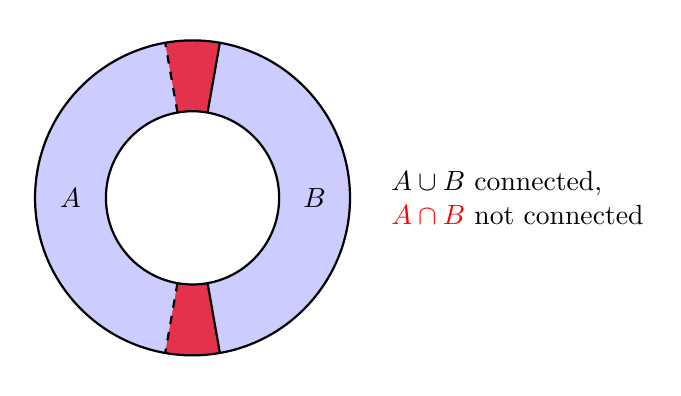
\begin{tikzpicture}
  % A: angles 80..280, B: angles -100..100 ; overlap at top and bottom
  \fill[blue, opacity=0.2] (80:2) arc (80:280:2) -- (280:1.1) arc (280:80:1.1) -- cycle;
  \fill[blue, opacity=0.2] (-100:2) arc (-100:100:2) -- (100:1.1) arc (100:-100:1.1) -- cycle;
  \fill[red, opacity=0.7] (80:2) arc (80:100:2) -- (100:1.1) arc (100:80:1.1) -- cycle;
  \fill[red, opacity=0.7] (260:2) arc (260:280:2) -- (280:1.1) arc (280:260:1.1) -- cycle;
  \draw[thick] (0,0) circle (2);
  \draw[thick] (0,0) circle (1.1);
  \draw[thick] (80:1.1) -- (80:2); \draw[thick] (280:1.1) -- (280:2);
  \draw[thick, dashed] (100:1.1) -- (100:2); \draw[thick, dashed] (260:1.1) -- (260:2);
  \node at (180:1.55) {$A$};
  \node at (0:1.55) {$B$};
  \node[right, align=left] at (2.4,0) {$A\cup B$ connected,\\ \textcolor{red}{$A\cap B$} not connected};
\end{tikzpicture}
